\documentclass[12pt, a4paper]{report}

% ─── Packages ───────────────────────────────────────────────────────────────
\usepackage[margin=2.5cm, headheight=25pt, top=2.8cm]{geometry}
\usepackage{graphicx}
\usepackage{xcolor}
\usepackage{titlesec}
\usepackage{titling}
\usepackage{fancyhdr}
\usepackage{enumitem}
\usepackage{listings}
\usepackage{booktabs}
\usepackage{tabularx}
\usepackage{array}
\usepackage{mdframed}
\usepackage{hyperref}
\usepackage{tcolorbox}
\usepackage{tikz}
\usepackage{amsmath}
\usepackage{parskip}
\usepackage[expansion=false]{microtype}
\usepackage{setspace}
\usepackage{caption}
\usepackage{float}

\tcbuselibrary{skins, breakable, listings}
\usetikzlibrary{shapes.geometric, arrows.meta, positioning, fit, backgrounds}

% ─── Colors ─────────────────────────────────────────────────────────────────
\definecolor{farmgreen}{RGB}{34, 120, 60}
\definecolor{soilbrown}{RGB}{101, 67, 33}
\definecolor{skyblue}{RGB}{30, 100, 180}
\definecolor{alertred}{RGB}{180, 30, 30}

% Code Block Specific Colors (Matching the provided light theme)
\definecolor{codebg}{RGB}{244, 244, 240}      % Light beige background
\definecolor{codepink}{RGB}{233, 30, 99}      % Pink for keywords (const, new, null, false)
\definecolor{codepurple}{RGB}{156, 39, 176}   % Purple for strings
\definecolor{codegray}{RGB}{150, 150, 150}    % Gray for line numbers and comments
\definecolor{codetext}{RGB}{0, 0, 0}          % Black for standard code text

% ─── Hyperref Setup ──────────────────────────────────────────────────────────
\hypersetup{
    colorlinks=true,
    linkcolor=farmgreen,
    urlcolor=skyblue,
    citecolor=farmgreen,
    pdfauthor={OOP II Project Team},
    pdftitle={Smart Farm Management System},
    pdfsubject={College Project Documentation}
}

% ─── Header & Footer ─────────────────────────────────────────────────────────
\pagestyle{fancy}
\fancyhf{}
\fancyhead[L]{\textcolor{farmgreen}{\textbf{Smart Farm Management System}}}
\fancyhead[R]{\textcolor{gray}{\small OOP II Project}}
\fancyfoot[C]{\textcolor{gray}{\thepage}}
\renewcommand{\headrulewidth}{0.4pt}
\renewcommand{\headrule}{\hbox to\headwidth{\color{farmgreen}\leaders\hrule height \headrulewidth\hfill}}

% ─── Section Title Styling ───────────────────────────────────────────────────
\titleformat{\chapter}[block]
  {\normalfont\LARGE\bfseries\color{farmgreen}}
  {\thechapter.}{12pt}{}
  [\vspace{2pt}{\color{farmgreen}\titlerule[1.5pt]}]

% Removes the massive default white space above chapters in report class
\titlespacing*{\chapter}{0pt}{-25pt}{20pt}

\titleformat{\section}
  {\normalfont\large\bfseries\color{soilbrown}}
  {\thesection}{10pt}{}

\titleformat{\subsection}
  {\normalfont\normalsize\bfseries\color{skyblue}}
  {\thesubsection}{8pt}{}

% ─── Code Listing Style ──────────────────────────────────────────────────────
\lstdefinestyle{javaStyle}{
    basicstyle=\color{codetext}\ttfamily\footnotesize,
    identifierstyle=\color{codetext},
    keywordstyle=\color{codepink},
    stringstyle=\color{codepurple},
    commentstyle=\color{codegray}\itshape,
    numberstyle=\tiny\color{codegray},
    numbers=left,
    numbersep=12pt,
    breaklines=true,
    frame=none,
    xleftmargin=24pt, % Pushes text right to keep line numbers inside the background box
    xrightmargin=6pt,
    showstringspaces=false,
    tabsize=4,
    language=Java,
    morekeywords={String, Thread, Socket, ServerSocket, Runnable, var, record, SensorHandler, IOException, SQLException, PreparedStatement, ResultSet, Connection, List, ArrayList, LocalDateTime, LocalDate, Date, HashMap, Map, Alert, Crop, Task, Worker, SensorReading, HarvestRecord, Platform, DashboardController, FXCollections, SimpleStringProperty, true, false, null},
}

\lstdefinestyle{cppStyle}{
    basicstyle=\color{codetext}\ttfamily\footnotesize,
    identifierstyle=\color{codetext},
    keywordstyle=\color{codepink},
    stringstyle=\color{codepurple},
    commentstyle=\color{codegray}\itshape,
    numberstyle=\tiny\color{codegray},
    numbers=left,
    numbersep=12pt,
    breaklines=true,
    frame=none,
    xleftmargin=24pt,
    xrightmargin=6pt,
    showstringspaces=false,
    tabsize=4,
    language=C++,
    morekeywords={WiFiClient, DHT, String, Serial, true, false, null}
}

\lstdefinestyle{sqlStyle}{
    basicstyle=\color{codetext}\ttfamily\footnotesize,
    identifierstyle=\color{codetext},
    keywordstyle=\color{codepink},
    stringstyle=\color{codepurple},
    commentstyle=\color{codegray}\itshape,
    numberstyle=\tiny\color{codegray},
    numbers=left,
    numbersep=12pt,
    breaklines=true,
    frame=none,
    xleftmargin=24pt,
    xrightmargin=6pt,
    showstringspaces=false,
    tabsize=4,
    language=SQL,
}

% ─── Custom Boxes ─────────────────────────────────────────────────────────────
\tcbset{
  notebox/.style={
    enhanced, breakable,
    colback=farmgreen!8,
    colframe=farmgreen,
    fonttitle=\bfseries,
    coltitle=white,
    attach boxed title to top left={yshift=-2mm, xshift=6mm},
    boxed title style={colback=farmgreen, rounded corners}
  },
  warnbox/.style={
    enhanced,
    colback=alertred!8,
    colframe=alertred,
    fonttitle=\bfseries,
    coltitle=white,
    attach boxed title to top left={yshift=-2mm, xshift=6mm},
    boxed title style={colback=alertred, rounded corners}
  },
  infobox/.style={
    enhanced, breakable,
    colback=skyblue!8,
    colframe=skyblue,
    fonttitle=\bfseries,
    coltitle=white,
    attach boxed title to top left={yshift=-2mm, xshift=6mm},
    boxed title style={colback=skyblue, rounded corners}
  }
}

% Custom tcblisting for exact match to the light-themed code blocks
\newtcblisting[auto counter, number within=chapter]{codeblock}[2]{
    listing only,
    breakable,
    pad at break=2mm,     % Prevents text from hitting the edge when page breaks
    bottomsep at break=5pt,
    topsep at break=5pt,
    colback=codebg,
    colframe=codebg,      % Invisible frame to match background
    coltext=codetext,     % Ensure text is black
    boxrule=0pt,          % No border
    arc=0pt,              % Sharp corners like the image
    outer arc=0pt,
    top=8pt,
    bottom=8pt,
    left=0pt,             % Space managed by listings' xleftmargin
    right=8pt,
    listing options={style=#1},
    after={\par\vspace{4pt}\begin{center}Listing \thetcbcounter: #2\end{center}\vspace{16pt}}
}

% ─── Document ─────────────────────────────────────────────────────────────────
\begin{document}

% ══════════════════════════════════════════════════════════════════════════════
%  TITLE PAGE
% ══════════════════════════════════════════════════════════════════════════════
\begin{titlepage}
\begin{tikzpicture}[remember picture, overlay]
    \fill[farmgreen] (current page.north west) rectangle ([yshift=-14cm]current page.north east);
    \fill[soilbrown] (current page.south west) rectangle ([yshift=1.8cm]current page.south east);
    \fill[farmgreen!30, opacity=0.4] ([xshift=12cm, yshift=-4cm]current page.north west) circle (5cm);
\end{tikzpicture}

\vspace*{1.5cm}
\begin{center}
    {\color{white}\fontsize{28}{34}\selectfont\bfseries Smart Farm}\\[4pt]
    {\color{white}\fontsize{22}{28}\selectfont\bfseries Management System}\\[10pt]
    {\color{white!80}\large A Full-Stack Java \& IoT College Project}

    \vspace{3.5cm}

    {\color{white}\rule{10cm}{1pt}}\\[18pt]
    {\large\bfseries\color{white} OOP II Module --- Project Documentation}\\[10pt]
    {\color{white!90} Covers: OOP Design $\cdot$ Multithreading $\cdot$ Networking $\cdot$ Database $\cdot$ JavaFX $\cdot$ IoT}\\[30pt]
    {\color{white}\rule{10cm}{1pt}}

    \vfill

    \begin{tabular}{rl}
        \textbf{Module:}   & Object-Oriented Programming II \\[4pt]
        \textbf{Hardware:} & ESP32 + DHT11 Sensor \\[4pt]
        \textbf{Stack:}    & Java, MySQL, JavaFX, Arduino C++ \\[4pt]
        \textbf{Year:}     & 2025 / 2026 \\
    \end{tabular}
\end{center}
\end{titlepage}

% ══════════════════════════════════════════════════════════════════════════════
\tableofcontents
\newpage

% ══════════════════════════════════════════════════════════════════════════════
\chapter{Introduction \& Project Overview}
% ══════════════════════════════════════════════════════════════════════════════

\section{What Is This Project?}

The \textbf{Smart Farm Management System} is a complete, real-world application that manages every aspect of running a farm --- from monitoring field conditions with physical sensors to tracking crops, assigning workers to tasks, logging harvests, and generating reports. It combines everything studied in the OOP II module into one coherent system.

The word ``smart'' is not decoration. The system does not just \emph{display} data --- it \emph{acts} on it. When the temperature in a field crosses a dangerous threshold, the system automatically generates an alert, creates a task (``irrigate Plot~3''), and assigns it to an available worker. Sensor data drives farm decisions.

\begin{tcolorbox}[notebox, title={The System in One Sentence}]
A physical sensor measures field conditions $\rightarrow$ a Java server processes the data $\rightarrow$ the system manages crops, workers, tasks, and harvests in a MySQL database $\rightarrow$ the farmer monitors and controls everything through a live JavaFX dashboard.
\end{tcolorbox}

\section{Core Capabilities}

The system provides six integrated capabilities:

\begin{enumerate}[leftmargin=*, label=\textbf{\arabic*.}]
    \item \textbf{Live Environmental Monitoring} --- real temperature and humidity data from physical IoT sensors, displayed in real time with historical charts.
    \item \textbf{Intelligent Alert System} --- automatic detection of dangerous conditions with severity levels that trigger actionable responses.
    \item \textbf{Crop \& Plot Management} --- full lifecycle tracking of crops from planting through growth stages to harvest, tied to specific farm plots.
    \item \textbf{Worker \& Task Management} --- assignment of workers to tasks on specific plots, with status tracking and workload balancing.
    \item \textbf{Harvest Logging \& Analytics} --- recording of yield quantity and quality grades, with comparison against expected output.
    \item \textbf{Report Export} --- CSV export of sensor logs, harvest summaries, and alert histories for external analysis.
\end{enumerate}

\section{Why Agriculture?}

Agriculture is an ideal domain because it demands every OOP~II concept simultaneously. Sensor data arrives continuously and from multiple sources, requiring \textbf{multithreading}. Different crops have different needs, requiring \textbf{inheritance and polymorphism}. Data must be persisted, requiring a \textbf{database}. The farmer needs a clear interface, requiring a \textbf{GUI}. And the physical sensor adds \textbf{networking} and \textbf{IoT} integration.

\section{OOP II Concepts Covered}

\begin{table}[H]
\centering
\renewcommand{\arraystretch}{1.5}
\begin{tabularx}{\textwidth}{>{\bfseries}l X l}
\toprule
\textbf{Concept} & \textbf{How It Appears in This Project} & \textbf{Module Topic} \\
\midrule
OOP Design        & \texttt{Crop}, \texttt{Plot}, \texttt{Worker}, \texttt{Alert} class hierarchies & Classes \& Inheritance \\
Interfaces        & \texttt{Runnable}, \texttt{DAOInterface}, \texttt{Exportable} & Abstraction \\
Multithreading    & One thread per ESP32 device, alert checker thread & Concurrency \\
Networking        & TCP socket between ESP32 and Java server & Java Sockets \\
Database (JDBC)   & MySQL storage of all readings, crops, alerts, tasks & JDBC \\
JavaFX GUI        & Live dashboard with charts, tables, forms, alerts & GUI Programming \\
File I/O          & CSV export of sensor logs and harvest reports & I/O Streams \\
Collections       & \texttt{List}, \texttt{Map}, \texttt{Queue} for managing data & Java Collections \\
Exception Handling & Network drops, DB errors, invalid sensor data & Error Handling \\
\bottomrule
\end{tabularx}
\caption{OOP II concepts and their role in the project}
\end{table}


% ══════════════════════════════════════════════════════════════════════════════
\chapter{System Architecture}
% ══════════════════════════════════════════════════════════════════════════════

\section{High-Level Overview}

The system consists of three physical components and four software layers:

\begin{enumerate}[leftmargin=*, label=\textbf{\arabic*.}]
    \item \textbf{The ESP32 Device} --- a microcontroller with a DHT11 sensor. Reads temperature and humidity, sends data over WiFi.
    \item \textbf{The Java Application} --- the server, business logic, and JavaFX dashboard all run here. It receives sensor data, manages farm operations, and presents the UI.
    \item \textbf{The MySQL Database} --- persistent storage for all data: readings, crops, plots, workers, tasks, alerts, and harvests.
\end{enumerate}

\vspace{10pt}

\begin{tcolorbox}[colback=lightgray, colframe=farmgreen, title={\textbf{System Flow Diagram}}, fonttitle=\bfseries\color{white}, attach boxed title to top left={yshift=-2mm, xshift=6mm}, boxed title style={colback=farmgreen}]
\begin{center}
\resizebox{\linewidth}{!}{
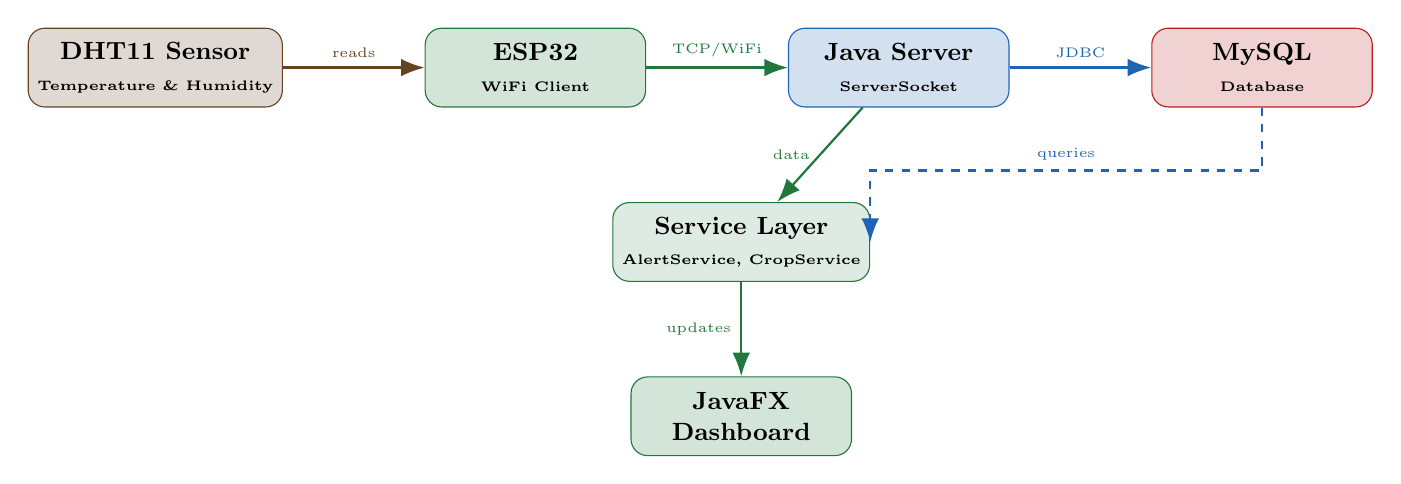
\begin{tikzpicture}[
    node distance=1.4cm and 1.8cm,
    box/.style={rectangle, rounded corners=6pt, draw, minimum width=2.8cm, minimum height=1cm, font=\small\bfseries, align=center},
    arrow/.style={-{Latex[length=3mm]}, thick}
]
    \node[box, fill=soilbrown!20, draw=soilbrown]       (dht)    {DHT11 Sensor\\{\tiny Temperature \& Humidity}};
    \node[box, fill=farmgreen!20, draw=farmgreen, right=of dht]  (esp)    {ESP32\\{\tiny WiFi Client}};
    \node[box, fill=skyblue!20, draw=skyblue, right=of esp]       (srv)    {Java Server\\{\tiny ServerSocket}};
    \node[box, fill=alertred!20, draw=alertred, right=of srv]     (db)     {MySQL\\{\tiny Database}};

    \node[box, fill=farmgreen!15, draw=farmgreen, below=1.2cm of srv, xshift=-2cm] (svc) {Service Layer\\{\tiny AlertService, CropService}};
    \node[box, fill=farmgreen!20, draw=farmgreen, below=1.2cm of svc] (ui) {JavaFX\\Dashboard};

    \draw[arrow, soilbrown] (dht) -- node[above, font=\tiny]{reads} (esp);
    \draw[arrow, farmgreen] (esp) -- node[above, font=\tiny]{TCP/WiFi} (srv);
    \draw[arrow, skyblue]   (srv) -- node[above, font=\tiny]{JDBC} (db);
    \draw[arrow, farmgreen] (srv) -- node[left, font=\tiny]{data} (svc);
    \draw[arrow, farmgreen] (svc) -- node[left, font=\tiny]{updates} (ui);
    \draw[arrow, skyblue, dashed] (db.south) -- ++(0,-0.8) -| node[near start, above, font=\tiny]{queries} (svc.east);
\end{tikzpicture}
}
\end{center}
\end{tcolorbox}

\section{Layered Architecture}

The software follows a strict layered architecture where each layer only communicates with the layer directly below it.

\begin{table}[H]
\centering
\renewcommand{\arraystretch}{1.6}
\begin{tabularx}{\textwidth}{>{\centering\bfseries}p{3.5cm} X >{\centering\arraybackslash}p{3.5cm}}
\toprule
\textbf{Layer} & \textbf{What Lives Here} & \textbf{Technology} \\
\midrule
Presentation Layer     & JavaFX screens, FXML files, UI controllers & JavaFX / FXML \\
Service Layer          & Business logic: alerts, crop lifecycle, task assignment, harvest analytics & Plain Java classes \\
Data Access Layer      & All database queries (DAO classes) & JDBC + MySQL \\
Infrastructure Layer   & Sockets, DB connection pool, ESP32 link & Java Sockets \\
\bottomrule
\end{tabularx}
\caption{The four layers and what lives in each one}
\end{table}

\textbf{The rule:} the Presentation layer never writes SQL. The DAO layer never decides whether to fire an alert. Each layer has one job.

\subsection{MVC in the JavaFX UI}

Inside the JavaFX layer, Model-View-Controller is used:
\begin{itemize}
    \item \textbf{Model} --- plain Java classes like \texttt{Crop}, \texttt{Worker}, \texttt{Alert} (data only)
    \item \textbf{View} --- \texttt{.fxml} files defining layout (no logic)
    \item \textbf{Controller} --- Java classes connecting the View to the Service layer
\end{itemize}

\subsection{Package Structure}

\begin{tcolorbox}[colback=codebg, colframe=gray, fontupper=\ttfamily\small\color{codetext}]
\begin{verbatim}
smartfarm/
+-- model/     ->  Crop.java, Plot.java, Worker.java, Task.java,
|                  Alert.java, SensorReading.java, HarvestRecord.java
+-- dao/       ->  CropDAO.java, PlotDAO.java, SensorDAO.java,
|                  AlertDAO.java, WorkerDAO.java, TaskDAO.java,
|                  HarvestDAO.java
+-- server/    ->  FarmServer.java, SensorHandler.java
+-- service/   ->  AlertService.java, SensorService.java,
|                  CropService.java, TaskService.java,
|                  HarvestService.java, WorkerService.java
+-- ui/        ->  DashboardController.java, CropController.java,
|                  WorkerController.java, AlertController.java,
|                  HarvestController.java
|                  dashboard.fxml, crops.fxml, workers.fxml,
|                  alerts.fxml, harvest.fxml
+-- util/      ->  DBConnection.java, CSVExporter.java,
|                  ThresholdConfig.java
\-- Main.java  ->  Entry point (starts server + opens dashboard)
\end{verbatim}
\end{tcolorbox}


% ══════════════════════════════════════════════════════════════════════════════
\chapter{The OOP Model --- Classes \& Relationships}
% ══════════════════════════════════════════════════════════════════════════════

This chapter defines every model class in the system. These are the building blocks that every other layer depends on.

\section{Plot}

A \texttt{Plot} represents a physical piece of land on the farm.

\begin{codeblock}{javaStyle}{Plot model class}
public class Plot {
    private int    plotId;
    private String name;
    private String location;
    private double sizeAcres;
    private String soilType;

    public Plot(String name, String location, double sizeAcres, String soilType) {
        this.name      = name;
        this.location  = location;
        this.sizeAcres = sizeAcres;
        this.soilType  = soilType;
    }

    // Getters and setters omitted for brevity

    @Override
    public String toString() {
        return String.format("Plot[%s] %s — %.1f acres, %s soil",
               plotId, name, sizeAcres, soilType);
    }
}
\end{codeblock}

\section{Crop}

A \texttt{Crop} is planted on a \texttt{Plot} and moves through a defined lifecycle.

\begin{codeblock}{javaStyle}{Crop model class with lifecycle enum}
public class Crop {
    public enum GrowthStage { PLANTED, GROWING, READY, HARVESTED }

    private int         cropId;
    private String      cropName;
    private LocalDate   plantingDate;
    private LocalDate   harvestDate;
    private GrowthStage growthStage;
    private int         plotId;
    private double      expectedYieldKg;

    public Crop(String cropName, LocalDate plantingDate, LocalDate harvestDate,
                int plotId, double expectedYieldKg) {
        this.cropName        = cropName;
        this.plantingDate    = plantingDate;
        this.harvestDate     = harvestDate;
        this.growthStage     = GrowthStage.PLANTED;
        this.plotId          = plotId;
        this.expectedYieldKg = expectedYieldKg;
    }

    /** Advance to next growth stage */
    public void advanceStage() {
        switch (growthStage) {
            case PLANTED  -> growthStage = GrowthStage.GROWING;
            case GROWING  -> growthStage = GrowthStage.READY;
            case READY    -> growthStage = GrowthStage.HARVESTED;
            case HARVESTED -> { /* already done */ }
        }
    }

    /** Check if crop is overdue for harvest */
    public boolean isOverdue() {
        return growthStage == GrowthStage.READY
            && LocalDate.now().isAfter(harvestDate);
    }

    // Getters and setters...
}
\end{codeblock}

\section{Worker and Task}

A \texttt{Worker} is a farm employee. A \texttt{Task} is a job assigned to a worker on a specific plot.

\begin{codeblock}{javaStyle}{Worker model class}
public class Worker {
    private int    workerId;
    private String name;
    private String role;
    private String phone;
    private int    activeTaskCount; // derived from task table

    public Worker(String name, String role, String phone) {
        this.name  = name;
        this.role  = role;
        this.phone = phone;
    }

    /** Check if worker is available (has fewer than 3 active tasks) */
    public boolean isAvailable() {
        return activeTaskCount < 3;
    }

    // Getters and setters...
}
\end{codeblock}

\begin{codeblock}{javaStyle}{Task model class with status lifecycle}
public class Task {
    public enum Status { PENDING, IN_PROGRESS, DONE }

    private int       taskId;
    private String    description;
    private Status    status;
    private LocalDate dueDate;
    private int       workerId;
    private int       plotId;
    private String    alertType; // null if manually created, set if auto-generated

    public Task(String description, LocalDate dueDate, int workerId, int plotId) {
        this.description = description;
        this.dueDate     = dueDate;
        this.workerId    = workerId;
        this.plotId      = plotId;
        this.status      = Status.PENDING;
    }

    public void advanceStatus() {
        switch (status) {
            case PENDING     -> status = Status.IN_PROGRESS;
            case IN_PROGRESS -> status = Status.DONE;
            case DONE        -> { /* already complete */ }
        }
    }

    public boolean isOverdue() {
        return status != Status.DONE && LocalDate.now().isAfter(dueDate);
    }

    // Getters and setters...
}
\end{codeblock}

\section{SensorReading}

\begin{codeblock}{javaStyle}{SensorReading model class}
public class SensorReading {
    private int           readingId;
    private String        deviceId;
    private float         temperature;
    private float         humidity;
    private LocalDateTime timestamp;

    public SensorReading(String deviceId, float temperature,
                         float humidity, LocalDateTime timestamp) {
        this.deviceId    = deviceId;
        this.temperature = temperature;
        this.humidity    = humidity;
        this.timestamp   = timestamp;
    }

    @Override
    public String toString() {
        return String.format("[%s] Device: %s | Temp: %.1f°C | Hum: %.1f%%",
               timestamp, deviceId, temperature, humidity);
    }
}
\end{codeblock}

\section{Alert}

\begin{codeblock}{javaStyle}{Alert model class}
public class Alert {
    public enum Severity { INFO, WARNING, CRITICAL }

    private int           alertId;
    private String        alertType;
    private Severity      severity;
    private String        message;
    private boolean       resolved;
    private LocalDateTime timestamp;
    private int           plotId;

    public Alert(String alertType, Severity severity, String message, int plotId) {
        this.alertType = alertType;
        this.severity  = severity;
        this.message   = message;
        this.plotId    = plotId;
        this.resolved  = false;
        this.timestamp = LocalDateTime.now();
    }

    public void resolve() {
        this.resolved = true;
    }
}
\end{codeblock}

\section{HarvestRecord}

\begin{codeblock}{javaStyle}{HarvestRecord model class}
public class HarvestRecord {
    public enum Grade { A, B, C }

    private int       recordId;
    private LocalDate harvestDate;
    private double    quantityKg;
    private Grade     grade;
    private int       cropId;

    public HarvestRecord(LocalDate harvestDate, double quantityKg,
                         Grade grade, int cropId) {
        this.harvestDate = harvestDate;
        this.quantityKg  = quantityKg;
        this.grade       = grade;
        this.cropId      = cropId;
    }
}
\end{codeblock}

\section{Class Relationship Summary}

\begin{table}[H]
\centering
\renewcommand{\arraystretch}{1.5}
\begin{tabularx}{\textwidth}{>{\bfseries}l X}
\toprule
\textbf{Relationship} & \textbf{Description} \\
\midrule
Plot has many Crops    & One plot can grow multiple crops over time \\
Plot has many Alerts   & Alerts are tied to a specific plot's sensor \\
Plot has many Tasks    & Work on a plot generates tasks \\
Worker has many Tasks  & A worker can be assigned multiple tasks \\
Task belongs to Plot   & Every task is performed on a specific plot \\
Crop has many Harvests & One crop can be harvested in batches \\
Alert can create Task  & A critical alert auto-generates a task \\
\bottomrule
\end{tabularx}
\caption{Class relationships in the system}
\end{table}


% ══════════════════════════════════════════════════════════════════════════════
\chapter{The Database Layer --- MySQL \& JDBC}
% ══════════════════════════════════════════════════════════════════════════════

\section{Database Schema}

Every piece of data is stored in MySQL. Nothing is lost when the application closes.

\begin{codeblock}{sqlStyle}{MySQL database schema}
-- Plots of land on the farm
CREATE TABLE plots (
    plot_id    INT PRIMARY KEY AUTO_INCREMENT,
    name       VARCHAR(100) NOT NULL,
    location   VARCHAR(200),
    size_acres DOUBLE,
    soil_type  VARCHAR(50)
);

-- Crops planted on each plot
CREATE TABLE crops (
    crop_id          INT PRIMARY KEY AUTO_INCREMENT,
    crop_name        VARCHAR(100) NOT NULL,
    planting_date    DATE,
    harvest_date     DATE,
    growth_stage     ENUM('PLANTED','GROWING','READY','HARVESTED'),
    expected_yield   DOUBLE,
    plot_id          INT,
    FOREIGN KEY (plot_id) REFERENCES plots(plot_id)
);

-- Every reading sent by an ESP32 device
CREATE TABLE sensor_readings (
    reading_id  INT PRIMARY KEY AUTO_INCREMENT,
    device_id   VARCHAR(100) NOT NULL,
    temperature FLOAT,
    humidity    FLOAT,
    timestamp   DATETIME DEFAULT CURRENT_TIMESTAMP
);

-- Alerts generated when thresholds are crossed
CREATE TABLE alerts (
    alert_id   INT PRIMARY KEY AUTO_INCREMENT,
    alert_type VARCHAR(50),
    severity   ENUM('INFO','WARNING','CRITICAL'),
    message    TEXT,
    resolved   BOOLEAN DEFAULT FALSE,
    timestamp  DATETIME DEFAULT CURRENT_TIMESTAMP,
    plot_id    INT,
    FOREIGN KEY (plot_id) REFERENCES plots(plot_id)
);

-- Farm workers
CREATE TABLE workers (
    worker_id INT PRIMARY KEY AUTO_INCREMENT,
    name      VARCHAR(100),
    role      VARCHAR(100),
    phone     VARCHAR(20)
);

-- Tasks assigned to workers
CREATE TABLE tasks (
    task_id     INT PRIMARY KEY AUTO_INCREMENT,
    description TEXT,
    status      ENUM('PENDING','IN_PROGRESS','DONE'),
    due_date    DATE,
    alert_type  VARCHAR(50), -- NULL if manual, set if auto-generated
    worker_id   INT,
    plot_id     INT,
    FOREIGN KEY (worker_id) REFERENCES workers(worker_id),
    FOREIGN KEY (plot_id)   REFERENCES plots(plot_id)
);

-- Harvest events
CREATE TABLE harvest_records (
    record_id    INT PRIMARY KEY AUTO_INCREMENT,
    harvest_date DATE,
    quantity_kg  DOUBLE,
    grade        ENUM('A','B','C'),
    crop_id      INT,
    FOREIGN KEY (crop_id) REFERENCES crops(crop_id)
);
\end{codeblock}

\section{DAO Pattern}

Each table has a corresponding DAO (Data Access Object) class. The DAO's only job is to talk to the database --- it contains no business logic. Below are two representative DAOs to show the pattern.

\begin{codeblock}{javaStyle}{SensorDAO --- saves and retrieves sensor readings}
public class SensorDAO {
    private final Connection conn = DBConnection.getInstance();

    public void saveReading(SensorReading reading) throws SQLException {
        String sql = "INSERT INTO sensor_readings (device_id, temperature, "
                   + "humidity, timestamp) VALUES (?, ?, ?, ?)";
        try (PreparedStatement stmt = conn.prepareStatement(sql)) {
            stmt.setString(1, reading.getDeviceId());
            stmt.setFloat (2, reading.getTemperature());
            stmt.setFloat (3, reading.getHumidity());
            stmt.setObject(4, reading.getTimestamp());
            stmt.executeUpdate();
        }
    }

    public List<SensorReading> getLast50Readings(String deviceId)
            throws SQLException {
        List<SensorReading> list = new ArrayList<>();
        String sql = "SELECT * FROM sensor_readings WHERE device_id = ? "
                   + "ORDER BY timestamp DESC LIMIT 50";
        try (PreparedStatement stmt = conn.prepareStatement(sql)) {
            stmt.setString(1, deviceId);
            ResultSet rs = stmt.executeQuery();
            while (rs.next()) {
                list.add(new SensorReading(
                    rs.getString("device_id"),
                    rs.getFloat("temperature"),
                    rs.getFloat("humidity"),
                    rs.getObject("timestamp", LocalDateTime.class)
                ));
            }
        }
        return list;
    }
}
\end{codeblock}

\begin{codeblock}{javaStyle}{CropDAO --- full CRUD for crops}
public class CropDAO {
    private final Connection conn = DBConnection.getInstance();

    public void addCrop(Crop crop) throws SQLException {
        String sql = "INSERT INTO crops (crop_name, planting_date, harvest_date, "
                   + "growth_stage, expected_yield, plot_id) "
                   + "VALUES (?, ?, ?, ?, ?, ?)";
        try (PreparedStatement stmt = conn.prepareStatement(sql)) {
            stmt.setString(1, crop.getCropName());
            stmt.setDate  (2, Date.valueOf(crop.getPlantingDate()));
            stmt.setDate  (3, Date.valueOf(crop.getHarvestDate()));
            stmt.setString(4, crop.getGrowthStage().name());
            stmt.setDouble(5, crop.getExpectedYieldKg());
            stmt.setInt   (6, crop.getPlotId());
            stmt.executeUpdate();
        }
    }

    public void updateGrowthStage(int cropId, Crop.GrowthStage stage)
            throws SQLException {
        String sql = "UPDATE crops SET growth_stage = ? WHERE crop_id = ?";
        try (PreparedStatement stmt = conn.prepareStatement(sql)) {
            stmt.setString(1, stage.name());
            stmt.setInt   (2, cropId);
            stmt.executeUpdate();
        }
    }

    public List<Crop> getCropsByPlot(int plotId) throws SQLException {
        List<Crop> list = new ArrayList<>();
        String sql = "SELECT * FROM crops WHERE plot_id = ? "
                   + "ORDER BY planting_date DESC";
        try (PreparedStatement stmt = conn.prepareStatement(sql)) {
            stmt.setInt(1, plotId);
            ResultSet rs = stmt.executeQuery();
            while (rs.next()) {
                Crop c = new Crop(
                    rs.getString("crop_name"),
                    rs.getDate("planting_date").toLocalDate(),
                    rs.getDate("harvest_date").toLocalDate(),
                    rs.getInt("plot_id"),
                    rs.getDouble("expected_yield")
                );
                c.setCropId(rs.getInt("crop_id"));
                // Set growth stage from DB value
                c.setGrowthStage(Crop.GrowthStage.valueOf(
                    rs.getString("growth_stage")));
                list.add(c);
            }
        }
        return list;
    }

    public List<Crop> getOverdueCrops() throws SQLException {
        List<Crop> list = new ArrayList<>();
        String sql = "SELECT * FROM crops WHERE growth_stage = 'READY' "
                   + "AND harvest_date < CURDATE()";
        try (PreparedStatement stmt = conn.prepareStatement(sql)) {
            ResultSet rs = stmt.executeQuery();
            while (rs.next()) {
                // same mapping as above...
            }
        }
        return list;
    }
}
\end{codeblock}

\begin{codeblock}{javaStyle}{TaskDAO --- task queries including workload counting}
public class TaskDAO {
    private final Connection conn = DBConnection.getInstance();

    public void addTask(Task task) throws SQLException {
        String sql = "INSERT INTO tasks (description, status, due_date, "
                   + "alert_type, worker_id, plot_id) "
                   + "VALUES (?, ?, ?, ?, ?, ?)";
        try (PreparedStatement stmt = conn.prepareStatement(sql)) {
            stmt.setString(1, task.getDescription());
            stmt.setString(2, task.getStatus().name());
            stmt.setDate  (3, Date.valueOf(task.getDueDate()));
            stmt.setString(4, task.getAlertType());
            stmt.setInt   (5, task.getWorkerId());
            stmt.setInt   (6, task.getPlotId());
            stmt.executeUpdate();
        }
    }

    public int getActiveTaskCount(int workerId) throws SQLException {
        String sql = "SELECT COUNT(*) FROM tasks "
                   + "WHERE worker_id = ? AND status != 'DONE'";
        try (PreparedStatement stmt = conn.prepareStatement(sql)) {
            stmt.setInt(1, workerId);
            ResultSet rs = stmt.executeQuery();
            rs.next();
            return rs.getInt(1);
        }
    }

    public List<Task> getOverdueTasks() throws SQLException {
        List<Task> list = new ArrayList<>();
        String sql = "SELECT * FROM tasks WHERE status != 'DONE' "
                   + "AND due_date < CURDATE()";
        try (PreparedStatement stmt = conn.prepareStatement(sql)) {
            ResultSet rs = stmt.executeQuery();
            while (rs.next()) {
                Task t = new Task(
                    rs.getString("description"),
                    rs.getDate("due_date").toLocalDate(),
                    rs.getInt("worker_id"),
                    rs.getInt("plot_id")
                );
                t.setTaskId(rs.getInt("task_id"));
                t.setStatus(Task.Status.valueOf(rs.getString("status")));
                list.add(t);
            }
        }
        return list;
    }
}
\end{codeblock}


% ══════════════════════════════════════════════════════════════════════════════
\chapter{The IoT Data Pipeline --- ESP32, Networking \& Server}
% ══════════════════════════════════════════════════════════════════════════════

This chapter covers the entire path data takes from the physical sensor to the Java application. It is one pipeline, presented as one chapter.

\section{The DHT11 Sensor}

The DHT11 is a small sensor (roughly \$2) that measures temperature (0--50\textdegree C, $\pm$2\textdegree C accuracy) and humidity (20--80\% RH, $\pm$5\% accuracy). It connects to the ESP32 with three wires: power (3.3V), ground, and data (GPIO~4).

\section{What the ESP32 Does}

The ESP32 runs a simple loop: connect to WiFi, connect to the Java server via TCP, read the DHT11 every 5~seconds, format the data as text, and send it. If the connection drops, it retries automatically.

The data format is a single text line:

\begin{tcolorbox}[colback=codebg, colframe=gray, fontupper=\ttfamily\color{codeyellow}]
DEVICE:plot1\_sensor,TEMP:27.50,HUM:63.20
\end{tcolorbox}

\section{ESP32 Firmware}

\begin{codeblock}{cppStyle}{ESP32 firmware --- sends DHT11 data to Java server}
#include <WiFi.h>
#include <DHT.h>

const char* WIFI_SSID     = "YourWiFiName";
const char* WIFI_PASSWORD = "YourWiFiPassword";
const char* SERVER_IP     = "192.168.1.100";
const int   SERVER_PORT   = 8080;
const char* DEVICE_ID     = "plot1_sensor";

#define DHT_PIN  4
#define DHT_TYPE DHT11

DHT dht(DHT_PIN, DHT_TYPE);
WiFiClient client;

void setup() {
    Serial.begin(115200);
    dht.begin();
    WiFi.begin(WIFI_SSID, WIFI_PASSWORD);
    while (WiFi.status() != WL_CONNECTED) {
        delay(500);
        Serial.print(".");
    }
    Serial.println("\nWiFi connected: " + WiFi.localIP().toString());
}

void loop() {
    if (!client.connected()) {
        if (!client.connect(SERVER_IP, SERVER_PORT)) {
            delay(5000);
            return;
        }
    }

    float temperature = dht.readTemperature();
    float humidity    = dht.readHumidity();

    if (isnan(temperature) || isnan(humidity)) {
        delay(2000);
        return;
    }

    String data = "DEVICE:" + String(DEVICE_ID)
                + ",TEMP:"  + String(temperature, 2)
                + ",HUM:"   + String(humidity, 2);
    client.println(data);
    delay(5000);
}
\end{codeblock}

\section{Java Server --- Receiving Connections}

The Java server uses \texttt{ServerSocket} to listen for ESP32 connections. Each connected device gets its own handler thread via an \texttt{ExecutorService}, so multiple sensors can connect simultaneously.

\begin{codeblock}{javaStyle}{FarmServer --- listens for ESP32 connections}
public class FarmServer {
    private static final int PORT = 8080;
    private ServerSocket serverSocket;
    private ExecutorService threadPool;

    public void start() {
        threadPool = Executors.newCachedThreadPool();
        try {
            serverSocket = new ServerSocket(PORT);
            System.out.println("Farm Server started on port " + PORT);

            while (true) {
                Socket deviceSocket = serverSocket.accept();
                System.out.println("Device connected: "
                    + deviceSocket.getInetAddress());
                threadPool.submit(new SensorHandler(deviceSocket));
            }
        } catch (IOException e) {
            System.err.println("Server error: " + e.getMessage());
        }
    }
}
\end{codeblock}

\section{SensorHandler --- Per-Device Thread}

\begin{codeblock}{javaStyle}{SensorHandler --- one thread per connected device}
public class SensorHandler implements Runnable {
    private final Socket socket;
    private final SensorService sensorService = new SensorService();

    public SensorHandler(Socket socket) {
        this.socket = socket;
    }

    @Override
    public void run() {
        try (BufferedReader reader = new BufferedReader(
                new InputStreamReader(socket.getInputStream()))) {
            String line;
            while ((line = reader.readLine()) != null) {
                SensorReading reading = parseReading(line);
                if (reading != null) {
                    sensorService.processReading(reading);
                }
            }
        } catch (IOException e) {
            System.out.println("Device disconnected: "
                + socket.getInetAddress());
        }
    }

    private SensorReading parseReading(String raw) {
        try {
            String[] parts = raw.split(",");
            String deviceId = parts[0].split(":")[1];
            float  temp     = Float.parseFloat(parts[1].split(":")[1]);
            float  hum      = Float.parseFloat(parts[2].split(":")[1]);
            return new SensorReading(deviceId, temp, hum,
                                     LocalDateTime.now());
        } catch (Exception e) {
            System.err.println("Bad data format: " + raw);
            return null;
        }
    }
}
\end{codeblock}


% ══════════════════════════════════════════════════════════════════════════════
\chapter{The Service Layer --- Business Logic}
% ══════════════════════════════════════════════════════════════════════════════

The service layer is where the system makes decisions. This is the ``brain'' of the Smart Farm. Each service class handles one domain of logic and uses the DAO layer to persist results.

\section{SensorService --- Processing Incoming Data}

When a reading arrives from the ESP32, \texttt{SensorService} coordinates the response: save it, check for alerts, and notify the UI.

\begin{codeblock}{javaStyle}{SensorService --- coordinates processing of each reading}
public class SensorService {
    private final SensorDAO  sensorDAO  = new SensorDAO();
    private final AlertService alertService = new AlertService();

    public void processReading(SensorReading reading) {
        try {
            // 1. Save to database
            sensorDAO.saveReading(reading);

            // 2. Determine which plot this sensor belongs to
            int plotId = resolvePlotId(reading.getDeviceId());

            // 3. Check for dangerous conditions
            alertService.checkAndAlert(reading, plotId);

            // 4. Notify the JavaFX dashboard (thread-safe)
            Platform.runLater(() ->
                DashboardController.getInstance().refreshSensorData()
            );
        } catch (SQLException e) {
            System.err.println("Failed to process reading: "
                + e.getMessage());
        }
    }

    private int resolvePlotId(String deviceId) {
        // Maps device IDs to plot IDs (e.g., "plot1_sensor" -> 1)
        return Integer.parseInt(
            deviceId.replaceAll("[^0-9]", ""));
    }
}
\end{codeblock}

\section{AlertService --- Intelligent Threshold Detection}

Every time a sensor reading arrives, \texttt{AlertService} checks it against configurable thresholds. When a threshold is breached, it creates an alert \textbf{and} auto-generates a task assigned to the least-busy available worker.

\begin{table}[H]
\centering
\renewcommand{\arraystretch}{1.5}
\begin{tabularx}{\textwidth}{l l l X}
\toprule
\textbf{Measurement} & \textbf{Threshold} & \textbf{Severity} & \textbf{Triggered Action} \\
\midrule
Temperature & $>$ 35\textdegree C      & CRITICAL & Alert + auto-task: ``Irrigate plot'' \\
Temperature & $>$ 30\textdegree C      & WARNING  & Alert only \\
Temperature & $<$ 5\textdegree C       & CRITICAL & Alert + auto-task: ``Cover crops'' \\
Humidity    & $<$ 30\%      & WARNING  & Alert + auto-task: ``Start irrigation'' \\
Humidity    & $>$ 85\%      & WARNING  & Alert only (fungal risk notice) \\
\bottomrule
\end{tabularx}
\caption{Alert thresholds and their triggered actions}
\end{table}

\begin{codeblock}{javaStyle}{AlertService --- checks thresholds, fires alerts, creates tasks}
public class AlertService {
    private final AlertDAO  alertDAO  = new AlertDAO();
    private final TaskService taskService = new TaskService();

    public void checkAndAlert(SensorReading reading, int plotId) {
        float temp = reading.getTemperature();
        float hum  = reading.getHumidity();

        // ── Temperature checks ─────────────────────────────────
        if (temp > 35.0f) {
            createAlertWithTask("HIGH_TEMP", "CRITICAL",
                "Extreme heat: " + temp + "C - crops may wilt!",
                plotId, "Irrigate plot immediately");
        } else if (temp > 30.0f) {
            createAlertOnly("HIGH_TEMP", "WARNING",
                "High temperature: " + temp + "C", plotId);
        } else if (temp < 5.0f) {
            createAlertWithTask("FROST_RISK", "CRITICAL",
                "Frost risk: " + temp + "C - protect crops!",
                plotId, "Cover crops with frost protection");
        }

        // ── Humidity checks ────────────────────────────────────
        if (hum < 30.0f) {
            createAlertWithTask("LOW_HUMIDITY", "WARNING",
                "Low humidity: " + hum + "% - irrigation needed",
                plotId, "Start irrigation system");
        } else if (hum > 85.0f) {
            createAlertOnly("HIGH_HUMIDITY", "WARNING",
                "High humidity: " + hum + "% - fungal risk",
                plotId);
        }
    }

    /** Creates alert AND auto-generates a task for it */
    private void createAlertWithTask(String type, String severity,
            String msg, int plotId, String taskDescription) {
        createAlertOnly(type, severity, msg, plotId);
        taskService.autoCreateTask(taskDescription, plotId, type);
    }

    private void createAlertOnly(String type, String severity,
            String msg, int plotId) {
        Alert alert = new Alert(type,
            Alert.Severity.valueOf(severity), msg, plotId);
        try {
            alertDAO.save(alert);
            System.out.println("[ALERT] " + severity + ": " + msg);
        } catch (SQLException e) {
            System.err.println("Failed to save alert: "
                + e.getMessage());
        }
    }
}
\end{codeblock}

\section{TaskService --- Automatic Task Assignment}

\texttt{TaskService} handles both manually created tasks and auto-generated tasks from alerts. For auto-tasks, it finds the least-busy available worker.

\begin{codeblock}{javaStyle}{TaskService --- assigns tasks to workers intelligently}
public class TaskService {
    private final TaskDAO   taskDAO   = new TaskDAO();
    private final WorkerDAO workerDAO = new WorkerDAO();

    /** Manually assign a task to a specific worker */
    public void createTask(String description, LocalDate dueDate,
                           int workerId, int plotId) {
        Task task = new Task(description, dueDate, workerId, plotId);
        try {
            taskDAO.addTask(task);
        } catch (SQLException e) {
            System.err.println("Failed to create task: "
                + e.getMessage());
        }
    }

    /** Auto-create a task from an alert — finds the best worker */
    public void autoCreateTask(String description, int plotId,
                               String alertType) {
        try {
            Worker worker = findLeastBusyWorker();
            if (worker == null) {
                System.out.println("No available workers for auto-task!");
                return;
            }

            Task task = new Task(description,
                LocalDate.now().plusDays(1), // due tomorrow
                worker.getWorkerId(), plotId);
            task.setAlertType(alertType);
            taskDAO.addTask(task);

            System.out.println("[AUTO-TASK] '" + description
                + "' assigned to " + worker.getName());
        } catch (SQLException e) {
            System.err.println("Failed to auto-create task: "
                + e.getMessage());
        }
    }

    /** Find the worker with the fewest active tasks */
    private Worker findLeastBusyWorker() throws SQLException {
        List<Worker> workers = workerDAO.getAllWorkers();
        Worker bestWorker = null;
        int minTasks = Integer.MAX_VALUE;

        for (Worker w : workers) {
            int count = taskDAO.getActiveTaskCount(w.getWorkerId());
            if (count < minTasks && count < 3) { // max 3 active tasks
                minTasks = count;
                bestWorker = w;
            }
        }
        return bestWorker;
    }

    /** Update task status */
    public void advanceTaskStatus(int taskId) {
        try {
            taskDAO.advanceStatus(taskId);
        } catch (SQLException e) {
            System.err.println("Failed to update task: "
                + e.getMessage());
        }
    }
}
\end{codeblock}

\section{CropService --- Crop Lifecycle Management}

\texttt{CropService} manages the full lifecycle of a crop and detects overdue harvests.

\begin{codeblock}{javaStyle}{CropService --- lifecycle management and overdue detection}
public class CropService {
    private final CropDAO    cropDAO    = new CropDAO();
    private final AlertDAO   alertDAO   = new AlertDAO();

    /** Plant a new crop on a specific plot */
    public void plantCrop(String name, LocalDate plantDate,
            LocalDate harvestDate, int plotId, double expectedYieldKg) {
        Crop crop = new Crop(name, plantDate, harvestDate,
                             plotId, expectedYieldKg);
        try {
            cropDAO.addCrop(crop);
        } catch (SQLException e) {
            System.err.println("Failed to plant crop: "
                + e.getMessage());
        }
    }

    /** Advance a crop to its next growth stage */
    public void advanceCropStage(int cropId) {
        try {
            Crop crop = cropDAO.getCropById(cropId);
            crop.advanceStage();
            cropDAO.updateGrowthStage(cropId, crop.getGrowthStage());
        } catch (SQLException e) {
            System.err.println("Failed to update crop stage: "
                + e.getMessage());
        }
    }

    /** Check all crops for overdue harvests and generate alerts */
    public void checkOverdueCrops() {
        try {
            List<Crop> overdue = cropDAO.getOverdueCrops();
            for (Crop c : overdue) {
                long daysLate = ChronoUnit.DAYS.between(
                    c.getHarvestDate(), LocalDate.now());
                Alert a = new Alert("OVERDUE_HARVEST",
                    Alert.Severity.WARNING,
                    c.getCropName() + " on plot " + c.getPlotId()
                    + " is " + daysLate + " days overdue for harvest",
                    c.getPlotId());
                alertDAO.save(a);
            }
        } catch (SQLException e) {
            System.err.println("Overdue check failed: "
                + e.getMessage());
        }
    }
}
\end{codeblock}

\section{HarvestService --- Yield Logging and Analytics}

\begin{codeblock}{javaStyle}{HarvestService --- records harvests and computes yield analytics}
public class HarvestService {
    private final HarvestDAO harvestDAO = new HarvestDAO();
    private final CropDAO    cropDAO    = new CropDAO();

    /** Record a harvest event */
    public void recordHarvest(int cropId, double quantityKg,
                              HarvestRecord.Grade grade) {
        HarvestRecord record = new HarvestRecord(
            LocalDate.now(), quantityKg, grade, cropId);
        try {
            harvestDAO.save(record);
            // Mark the crop as harvested
            cropDAO.updateGrowthStage(cropId,
                Crop.GrowthStage.HARVESTED);
        } catch (SQLException e) {
            System.err.println("Failed to record harvest: "
                + e.getMessage());
        }
    }

    /** Get yield summary for a plot: total kg, grade distribution */
    public Map<String, Object> getPlotYieldSummary(int plotId) {
        Map<String, Object> summary = new HashMap<>();
        try {
            List<HarvestRecord> records =
                harvestDAO.getByPlot(plotId);
            double totalKg = records.stream()
                .mapToDouble(HarvestRecord::getQuantityKg).sum();
            long gradeA = records.stream()
                .filter(r -> r.getGrade() == HarvestRecord.Grade.A)
                .count();
            long gradeB = records.stream()
                .filter(r -> r.getGrade() == HarvestRecord.Grade.B)
                .count();
            long gradeC = records.stream()
                .filter(r -> r.getGrade() == HarvestRecord.Grade.C)
                .count();

            summary.put("totalKg", totalKg);
            summary.put("gradeA", gradeA);
            summary.put("gradeB", gradeB);
            summary.put("gradeC", gradeC);
            summary.put("harvestCount", records.size());
        } catch (SQLException e) {
            System.err.println("Failed to get summary: "
                + e.getMessage());
        }
        return summary;
    }

    /** Compare actual yield vs expected yield */
    public double getYieldEfficiency(int cropId) {
        try {
            Crop crop = cropDAO.getCropById(cropId);
            double actualTotal = harvestDAO.getTotalYield(cropId);
            if (crop.getExpectedYieldKg() > 0) {
                return (actualTotal / crop.getExpectedYieldKg()) * 100;
            }
        } catch (SQLException e) {
            System.err.println("Yield calculation failed: "
                + e.getMessage());
        }
        return 0.0;
    }
}
\end{codeblock}


% ══════════════════════════════════════════════════════════════════════════════
\chapter{The JavaFX Dashboard}
% ══════════════════════════════════════════════════════════════════════════════

The dashboard is the farmer's single point of control for the entire system. It uses JavaFX with FXML layout files and controller classes.

\section{Dashboard Layout}

The main dashboard screen is divided into four panels:

\begin{enumerate}[leftmargin=*, label=\textbf{\arabic*.}]
    \item \textbf{Live Sensor Panel} --- current temperature and humidity with a real-time line chart updated every 5 seconds.
    \item \textbf{Alert Panel} --- active alerts colour-coded by severity (green for INFO, orange for WARNING, red for CRITICAL) with a ``Resolve'' button.
    \item \textbf{Farm Overview} --- summary cards showing total plots, active crops, pending tasks, and unresolved alerts.
    \item \textbf{Navigation Sidebar} --- links to Crops, Workers, Tasks, Harvest, and Export screens.
\end{enumerate}

\section{Live Chart --- Thread-Safe UI Updates}

Because sensor data arrives on the server thread, UI updates must be marshalled to the JavaFX Application Thread using \texttt{Platform.runLater()}.

\begin{codeblock}{javaStyle}{DashboardController --- live chart updates}
public class DashboardController {
    @FXML private LineChart<String, Number> tempChart;
    @FXML private LineChart<String, Number> humChart;
    @FXML private Label currentTemp;
    @FXML private Label currentHum;
    @FXML private TableView<Alert> alertTable;
    @FXML private Label totalPlots;
    @FXML private Label activeCrops;
    @FXML private Label pendingTasks;

    private XYChart.Series<String, Number> tempSeries;
    private XYChart.Series<String, Number> humSeries;
    private final SensorDAO sensorDAO = new SensorDAO();
    private static DashboardController instance;

    public static DashboardController getInstance() {
        return instance;
    }

    @FXML
    public void initialize() {
        instance = this;
        tempSeries = new XYChart.Series<>();
        tempSeries.setName("Temperature");
        tempChart.getData().add(tempSeries);

        humSeries = new XYChart.Series<>();
        humSeries.setName("Humidity");
        humChart.getData().add(humSeries);

        refreshSensorData();
        refreshOverview();
    }

    /** Called from SensorService via Platform.runLater() */
    public void refreshSensorData() {
        try {
            List<SensorReading> readings =
                sensorDAO.getLast50Readings("plot1_sensor");
            if (!readings.isEmpty()) {
                SensorReading latest = readings.get(0);
                currentTemp.setText(
                    String.format("%.1f C", latest.getTemperature()));
                currentHum.setText(
                    String.format("%.1f%%", latest.getHumidity()));
            }

            // Update chart series
            tempSeries.getData().clear();
            humSeries.getData().clear();
            DateTimeFormatter fmt =
                DateTimeFormatter.ofPattern("HH:mm:ss");
            for (SensorReading r : readings) {
                String time = r.getTimestamp().format(fmt);
                tempSeries.getData().add(
                    new XYChart.Data<>(time, r.getTemperature()));
                humSeries.getData().add(
                    new XYChart.Data<>(time, r.getHumidity()));
            }
        } catch (SQLException e) {
            System.err.println("Failed to refresh sensor data");
        }
    }
}
\end{codeblock}

\section{Alert Panel with Resolve Action}

\begin{codeblock}{javaStyle}{AlertController --- display and resolve alerts}
public class AlertController {
    @FXML private TableView<Alert> alertTable;
    @FXML private TableColumn<Alert, String> severityCol;
    @FXML private TableColumn<Alert, String> messageCol;
    @FXML private TableColumn<Alert, String> timeCol;

    private final AlertDAO alertDAO = new AlertDAO();

    @FXML
    public void initialize() {
        severityCol.setCellValueFactory(
            data -> new SimpleStringProperty(
                data.getValue().getSeverity().name()));
        messageCol.setCellValueFactory(
            data -> new SimpleStringProperty(
                data.getValue().getMessage()));
        timeCol.setCellValueFactory(
            data -> new SimpleStringProperty(
                data.getValue().getTimestamp()
                    .format(DateTimeFormatter.ofPattern("dd/MM HH:mm"))));

        // Colour rows by severity
        alertTable.setRowFactory(tv -> new TableRow<>() {
            @Override
            protected void updateItem(Alert alert, boolean empty) {
                super.updateItem(alert, empty);
                if (alert == null || empty) {
                    setStyle("");
                } else {
                    switch (alert.getSeverity()) {
                        case CRITICAL -> setStyle(
                            "-fx-background-color: #ffcccc;");
                        case WARNING  -> setStyle(
                            "-fx-background-color: #fff3cd;");
                        case INFO     -> setStyle(
                            "-fx-background-color: #d4edda;");
                    }
                }
            }
        });
        refreshAlerts();
    }

    @FXML
    private void onResolveClicked() {
        Alert selected = alertTable.getSelectionModel()
                                   .getSelectedItem();
        if (selected != null) {
            try {
                alertDAO.markResolved(selected.getAlertId());
                refreshAlerts();
            } catch (SQLException e) {
                System.err.println("Failed to resolve alert");
            }
        }
    }

    private void refreshAlerts() {
        try {
            List<Alert> alerts = alertDAO.getUnresolved();
            alertTable.setItems(
                FXCollections.observableArrayList(alerts));
        } catch (SQLException e) {
            System.err.println("Failed to load alerts");
        }
    }
}
\end{codeblock}


% ══════════════════════════════════════════════════════════════════════════════
\chapter{CSV Export --- File I/O}
% ══════════════════════════════════════════════════════════════════════════════

The system can export data to CSV files for external analysis (e.g.\ in Excel). The \texttt{CSVExporter} utility handles formatting and writing.

\begin{codeblock}{javaStyle}{CSVExporter --- generic CSV export utility}
public class CSVExporter {

    /** Export sensor readings to CSV */
    public static void exportSensorData(List<SensorReading> readings,
                                        String filePath) throws IOException {
        try (BufferedWriter writer = new BufferedWriter(
                new FileWriter(filePath))) {
            // Header
            writer.write("Timestamp,DeviceID,Temperature,Humidity");
            writer.newLine();

            // Data rows
            DateTimeFormatter fmt =
                DateTimeFormatter.ofPattern("yyyy-MM-dd HH:mm:ss");
            for (SensorReading r : readings) {
                writer.write(String.format("%s,%s,%.2f,%.2f",
                    r.getTimestamp().format(fmt),
                    r.getDeviceId(),
                    r.getTemperature(),
                    r.getHumidity()));
                writer.newLine();
            }
        }
    }

    /** Export harvest records to CSV */
    public static void exportHarvestData(List<HarvestRecord> records,
                                         String filePath) throws IOException {
        try (BufferedWriter writer = new BufferedWriter(
                new FileWriter(filePath))) {
            writer.write("HarvestDate,CropID,QuantityKg,Grade");
            writer.newLine();

            for (HarvestRecord r : records) {
                writer.write(String.format("%s,%d,%.2f,%s",
                    r.getHarvestDate(),
                    r.getCropId(),
                    r.getQuantityKg(),
                    r.getGrade().name()));
                writer.newLine();
            }
        }
    }
}
\end{codeblock}


% ══════════════════════════════════════════════════════════════════════════════
\chapter{Build Roadmap}
% ══════════════════════════════════════════════════════════════════════════════

\section{Suggested Build Order}

Build the system in stages so that something is always working and testable at each step.

\begin{tcolorbox}[infobox, title={Stage 1 --- Foundation (Day 1)}]
\begin{itemize}[noitemsep]
    \item Set up the MySQL database and run the schema script
    \item Create \texttt{DBConnection.java} utility (Singleton pattern)
    \item Write all model classes: \texttt{Plot}, \texttt{Crop}, \texttt{Worker}, \texttt{Task}, \texttt{Alert}, \texttt{SensorReading}, \texttt{HarvestRecord}
    \item Write all DAO classes and test each one
\end{itemize}
\end{tcolorbox}

\begin{tcolorbox}[infobox, title={Stage 2 --- Farm Management Core (Day 2-3)}]
\begin{itemize}[noitemsep]
    \item Build \texttt{CropService} and \texttt{TaskService} with business logic
    \item Build Crop \& Plot management UI screens in JavaFX --- full CRUD working
    \item Build Worker \& Task management UI with status advancement
    \item Connect all screens to the service layer
\end{itemize}
\end{tcolorbox}

\begin{tcolorbox}[infobox, title={Stage 3 --- Networking \& IoT Pipeline (Day 4)}]
\begin{itemize}[noitemsep]
    \item Build \texttt{FarmServer.java} and \texttt{SensorHandler.java}
    \item Test with a simulated Java client (no ESP32 yet)
    \item Verify data flows: client $\rightarrow$ server $\rightarrow$ database
\end{itemize}
\end{tcolorbox}

\begin{tcolorbox}[infobox, title={Stage 4 --- ESP32 Integration (Day 4)}]
\begin{itemize}[noitemsep]
    \item Wire the DHT11 to the ESP32 (3 wires)
    \item Upload the firmware with your WiFi and server IP
    \item Confirm real readings appear in the database
\end{itemize}
\end{tcolorbox}

\begin{tcolorbox}[notebox, title={Stage 5 --- Alert System \& Auto-Tasks (Day 5)}]
\begin{itemize}[noitemsep]
    \item Implement \texttt{AlertService} with threshold checking
    \item Implement auto-task creation from critical alerts
    \item Connect alerts to the dashboard UI with colour-coded severity
\end{itemize}
\end{tcolorbox}

\begin{tcolorbox}[notebox, title={Stage 6 --- Full Dashboard (Day 6)}]
\begin{itemize}[noitemsep]
    \item Build the live sensor chart using \texttt{Platform.runLater()}
    \item Build the alert panel with resolve button
    \item Build the farm overview cards (summary statistics)
    \item Connect all screens with navigation sidebar
\end{itemize}
\end{tcolorbox}

\begin{tcolorbox}[notebox, title={Stage 7 --- Harvest, Export \& Polish (Day 7)}]
\begin{itemize}[noitemsep]
    \item Build Harvest logging screen with yield analytics
    \item Implement CSV export for sensor and harvest data
    \item Add error handling for network drops and DB failures
    \item Implement overdue crop detection
    \item Write final documentation
\end{itemize}
\end{tcolorbox}


% ══════════════════════════════════════════════════════════════════════════════
\chapter{Technology Stack \& Hardware Reference}
% ══════════════════════════════════════════════════════════════════════════════

\section{Technology Stack}

\begin{table}[H]
\centering
\renewcommand{\arraystretch}{1.6}
\begin{tabularx}{\textwidth}{>{\bfseries}l l X}
\toprule
\textbf{Component} & \textbf{Technology} & \textbf{Purpose} \\
\midrule
Language         & Java 17+            & Main application language \\
GUI              & JavaFX              & Dashboard and all UI screens \\
Database         & MySQL 8             & Persistent storage \\
DB Driver        & JDBC (mysql-connector-j) & Java to MySQL communication \\
Server           & Java ServerSocket   & Receives ESP32 connections \\
Concurrency      & ExecutorService     & Thread pool for device handlers \\
Microcontroller  & ESP32               & Field device with WiFi \\
Sensor           & DHT11               & Measures temperature \& humidity \\
Firmware         & Arduino C++         & ESP32 programming language \\
IDE (Java)       & IntelliJ IDEA / Eclipse & Java development \\
IDE (ESP32)      & Arduino IDE         & ESP32 firmware development \\
Build Tool       & Maven or Gradle     & Java dependency management \\
\bottomrule
\end{tabularx}
\caption{Full technology stack}
\end{table}

\section{Hardware Shopping List}

\begin{table}[H]
\centering
\renewcommand{\arraystretch}{1.5}
\begin{tabularx}{\textwidth}{l X l}
\toprule
\textbf{Component} & \textbf{Description} & \textbf{Price (approx)} \\
\midrule
ESP32 Dev Board  & Microcontroller with built-in WiFi & \$5--10 \\
DHT11 Sensor     & Temperature \& humidity sensor & \$1--2 \\
Breadboard       & For prototyping connections & \$2--3 \\
Jumper Wires     & Male-to-male, assorted & \$2 \\
USB Cable        & Micro-USB for ESP32 (often included) & --- \\
\midrule
\textbf{Total}   & & \textbf{\$10--17} \\
\bottomrule
\end{tabularx}
\caption{Full hardware shopping list}
\end{table}

\section{DHT11 to ESP32 Wiring}

\begin{table}[H]
\centering
\renewcommand{\arraystretch}{1.5}
\begin{tabular}{ccc}
\toprule
\textbf{DHT11 Pin} & \textbf{ESP32 Pin} & \textbf{Description} \\
\midrule
VCC (Pin 1) & 3.3V       & Power \\
Data (Pin 2)& GPIO 4     & Data signal \\
GND (Pin 4) & GND        & Ground \\
\bottomrule
\end{tabular}
\caption{DHT11 to ESP32 wiring (only 3 wires needed)}
\end{table}

\begin{tcolorbox}[warnbox, title={Important Note}]
The DHT11 module (on a small PCB with 3 pins) has the pull-up resistor built in. If you have the raw sensor (4 pins), add a 10k$\Omega$ resistor between VCC and the Data pin.
\end{tcolorbox}


% ══════════════════════════════════════════════════════════════════════════════
\chapter{Conclusion}
% ══════════════════════════════════════════════════════════════════════════════

The Smart Farm Management System demonstrates mastery of every topic in the OOP~II module --- not as isolated features, but as an integrated system where each part depends on the others.

The sensor is not the project --- it is the starting point. The real value is what the system \emph{does} with the data: it detects dangerous conditions, automatically creates tasks, assigns them to workers, tracks crop lifecycles, logs harvests, computes yield efficiency, and exports reports. Every OOP~II concept has a clear, meaningful role:

\begin{itemize}
    \item \textbf{OOP design} --- seven model classes with enums, lifecycle methods, and clear relationships.
    \item \textbf{Multithreading} --- one thread per connected sensor device.
    \item \textbf{Networking} --- TCP socket between the ESP32 and Java server.
    \item \textbf{JDBC and MySQL} --- seven tables storing every piece of farm data.
    \item \textbf{Business logic} --- five service classes that make intelligent decisions.
    \item \textbf{JavaFX} --- a live dashboard with charts, tables, alerts, and CRUD screens.
    \item \textbf{File I/O} --- CSV export for external analysis.
\end{itemize}

The demo moment ties it all together: hold the DHT11 sensor, breathe on it, and watch the dashboard chart spike, a humidity alert fire, an auto-task get assigned to a worker, and the task appear on the task board --- all in real time, end to end.

\vspace{20pt}
\begin{tcolorbox}[notebox, title={Getting Started}]
\begin{enumerate}[noitemsep]
    \item Set up MySQL and run the schema script from Chapter~4.
    \item Create the Java project with the package structure from Chapter~2.
    \item Write all model classes (Chapter~3) and test the DAO layer first.
    \item Order the ESP32 and DHT11 (1--2 weeks to arrive).
    \item Build the service layer and management screens while waiting for hardware.
    \item Integrate the sensor last --- everything else should already work.
\end{enumerate}
\end{tcolorbox}

\end{document}